\documentclass[english,10pt,a4paper]{article}
\usepackage{tcolorbox}
\usepackage{ulem} %math
\usepackage{amsmath}
\usepackage{amsfonts}
\usepackage{amssymb}
\usepackage{graphicx}
\usepackage{enumerate}


%Create a box for theorems
%\begin{theo}[titel] %optional
%tekst
%\end{theo}
\newenvironment{theo}[1][Vigtigt]{%
\begin{tcolorbox}[colback=green!5,colframe=green!40!black,title=\textbf{#1}]
}{%
\end{tcolorbox}
}




%Create a square matrix
%\begin{ArgMat}{2}
%21 & 22 & 23 \\  
%a & b & c
%\end{ArgMat}
%
% Info: http://tex.stackexchange.com/questions/2233/whats-the-best-way-make-an-augmented-coefficient-matrix
%
\newenvironment{ArgMat}{%
$
  \left[\begin{array}{@{}*{100}{r}r@{}}
}{%
  \end{array}\right]
  $
}

\newenvironment{deter}{%
$
  \left|\begin{array}{@{}*{100}{r}r@{}}
}{%
  \end{array}\right|
  $
}


%Create multiple lines with holes
%\begin{SysEqu}
%x_1 && &- &5x_3 &+ &2x_4=& 1 \\
%x_1 &+ &x_2 &+ &x_3 && =& 4 \\
%&&&&&&0 =& 0
%\end{SysEqu}
\newenvironment{SysEqu}{%
$  \setlength\arraycolsep{0.1em}
  \begin{array}{@{}*{100}{r}r@{}}
}{%
  \end{array}$
}

%Create solution for x_1, x_n...
%\begin{solu}
%x_1 &= d \\
%x_2 &= e \\
%x_3 &= s
%\end{solu}
\newenvironment{solu}{%
$
  \setlength\arraycolsep{0.1em}
  \left\{\begin{array}{@{}*{100}{r}r@{}}
}{%
  \end{array}\right.
$
}

\usepackage{lastpage}


\newcommand{\HRule}{\rule{\linewidth}{0.8mm}}

%Tekst i fotter
\newcommand{\footerText}{\thepage\xspace /\pageref{LastPage}}
\newcommand{\ProjectName}{433 MHz styring af AeroQuad}


\chapterstyle{hangnum}




\nouppercaseheads
\makepagestyle{mystyle} 

\makeevenhead{mystyle}{}{\\ \leftmark}{} 
\makeoddhead{mystyle}{}{\\ \leftmark}{} 
\makeevenfoot{mystyle}{}{\footerText}{} 
\makeoddfoot{mystyle}{}{\footerText}{} 
\makeatletter
\makepsmarks{mystyle}{% Overskriften på sidehovedet
  \createmark{chapter}{left}{shownumber}{\@chapapp\ }{.\ }} 
\makeatother
\makefootrule{mystyle}{\textwidth}{\normalrulethickness}{0.4pt}
\makeheadrule{mystyle}{\textwidth}{\normalrulethickness}

\makepagestyle{plain}
\makeevenhead{plain}{}{}{}
\makeoddhead{plain}{}{}{}
\makeevenfoot{plain}{}{\footerText}{}
\makeoddfoot{plain}{}{\footerText}{}
\makefootrule{plain}{\textwidth}{\normalrulethickness}{0.4pt}

\pagestyle{mystyle}

%%----------------------------------------------------------------------
%
%%Redefining chapter style
%%\renewcommand\chapterheadstart{\vspace*{\beforechapskip}}
%\renewcommand\chapterheadstart{\vspace*{10pt}}
%\renewcommand\printchaptername{\chapnamefont }%\@chapapp}
%\renewcommand\chapternamenum{\space}
%\renewcommand\printchapternum{\chapnumfont \thechapter}
%\renewcommand\afterchapternum{\space: }%\par\nobreak\vskip \midchapskip}
%\renewcommand\printchapternonum{}
%\renewcommand\printchaptertitle[1]{\chaptitlefont #1}
\setlength{\beforechapskip}{0pt} 
\setlength{\afterchapskip}{0pt} 
%\setlength{\voffset}{0pt} 
\setlength{\headsep}{25pt}
%\setlength{\topmargin}{35pt}
%%\setlength{\headheight}{102pt}
%\setlength{\textheight}{302pt}
\renewcommand\afterchaptertitle{\par\nobreak\vskip \afterchapskip}
%%----------------------------------------------------------------------




%Sidehoved og -fod pakke
%Margin
\usepackage[left=2cm,right=2cm,top=2.5cm,bottom=2cm]{geometry}
\usepackage{lastpage}



%%URL kommandoer og sidetal farve
%%Kaldes med \url{www...}
%\usepackage{color} %Skal også bruges
\usepackage{hyperref}
\hypersetup{ 
	colorlinks	= true, 	% false: boxed links; true: colored links
    urlcolor	= blue,		% color of external links
    linkcolor	= black, 	% color of page numbers
    citecolor	= blue,
}



%Mellemrum mellem linjerne    
\linespread{1.5}


%Seperated files
%--------------------------------------------------
%Opret filer således:
%\documentclass[Navn-på-hovedfil]{subfiles}
%\begin{document}
% Indmad
%\end{document}
%
% I hovedfil inkluderes således:
% \subfile{navn-på-subfil}
%--------------------------------------------------
\usepackage{subfiles}

%Prevent wierd placement of figures
%\usepackage[section]{placeins}

%Standard sti at søge efter billeder
%--------------------------------------------------
%\begin{figure}[hbtp]
%\centering
%\includegraphics[scale=1]{filnavn-for-png}
%\caption{Titel}
%\label{fig:referenceNavn}
%\end{figure}
%--------------------------------------------------
\usepackage{graphicx}
\usepackage{subcaption}
\usepackage{float}
\graphicspath{{../Figures/}}

%Speciel skrift for enkelt linje kode
%--------------------------------------------------
%Udskriver med fonten 'Courier'
%Mere info her: http://tex.stackexchange.com/questions/25249/how-do-i-use-a-particular-font-for-a-small-section-of-text-in-my-document
%Eksempel: Funktionen \code{void Hello()} giver et output
%--------------------------------------------------
\newcommand{\code}[1]{{\fontfamily{pcr}\selectfont #1}}


% Følgende er til koder.
%----------------------------------------------------------
%\begin{lstlisting}[caption=Overskrift på boks, style=Code-C++, label=lst:referenceLabel]
%public void hello(){}
%\end{lstlisting}
%----------------------------------------------------------

%Exstra space
\usepackage{xspace}
%Navn på bokse efterfulgt af \xspace (hvis det skal være mellemrum
%gives det med denne udvidelse. Ellers ingen mellemrum.
\newcommand{\codeTitle}{Kodeudsnit\xspace}

%Pakker der skal bruges til lstlisting
\usepackage{listings}
\usepackage{color}
\usepackage{textcomp}
\definecolor{listinggray}{gray}{0.9}
\definecolor{lbcolor}{rgb}{0.9,0.9,0.9}
\renewcommand{\lstlistingname}{\codeTitle}
\lstdefinestyle{Code}
{
	keywordstyle	= \bfseries\ttfamily\color[rgb]{0,0,1},
	identifierstyle	= \ttfamily,
	commentstyle	= \color[rgb]{0.133,0.545,0.133},
	stringstyle		= \ttfamily\color[rgb]{0.627,0.126,0.941},
	showstringspaces= false,
	basicstyle		= \small,
	numberstyle		= \footnotesize,
%	numbers			= left, % Tal? Udkommenter hvis ikke
	stepnumber		= 2,
	numbersep		= 6pt,
	tabsize			= 2,
	breaklines		= true,
	prebreak 		= \raisebox{0ex}[0ex][0ex]{\ensuremath{\hookleftarrow}},
	breakatwhitespace= false,
%	aboveskip		= {1.5\baselineskip},
  	columns			= fixed,
  	upquote			= true,
  	extendedchars	= true,
 	backgroundcolor = \color{lbcolor},
	lineskip		= 1pt,
%	xleftmargin		= 17pt,
%	framexleftmargin= 17pt,
	framexrightmargin	= 0pt, %6pt
%	framexbottommargin	= 4pt,
}

%Bredde der bruges til indryk
%Den skal være 6 pt mindre
\usepackage{calc}
\newlength{\mywidth}
\setlength{\mywidth}{\textwidth-6pt}


% Forskellige styles for forskellige kodetyper
\usepackage{caption}
\DeclareCaptionFont{white}{\color{white}}
\DeclareCaptionFormat{listing}%
{\colorbox[cmyk]{0.43, 0.35, 0.35,0.35}{\parbox{\mywidth}{\hspace{5pt}#1#2#3}}}
\captionsetup[lstlisting]
{
	format			= listing,
	labelfont		= white,
	textfont		= white, 
	singlelinecheck	= false, 
	width			= \mywidth,
	margin			= 0pt, 
	font			= {bf,footnotesize}
}

\lstdefinestyle{Code-C} {language=C, style=Code}
\lstdefinestyle{Code-Java} {language=Java, style=Code}
\lstdefinestyle{Code-C++} {language=[Visual]C++, style=Code}
\lstdefinestyle{Code-VHDL} {language=VHDL, style=Code}
\lstdefinestyle{Code-Bash} {language=Bash, style=Code}

%Text typesetting
%--------------------------------------------------------
%\usepackage{baskervald}
\usepackage{lmodern}
\usepackage[T1]{fontenc}              
\usepackage[utf8]{inputenc}         
\usepackage[english]{babel}       

\setlength{\parindent}{0pt}
\nonzeroparskip

%\setaftersubsecskip{1sp}
%\setaftersubsubsecskip{1sp}
 


%Dybde på indholdsfortegnelse
%----------------------------------------------------------
%Chapter, section, subsection, subsubsection
%----------------------------------------------------------
\setcounter{secnumdepth}{3}
\setcounter{tocdepth}{3}


%Tables
%----------------------------------------------------------
\usepackage{tabularx}
\usepackage{array}
\usepackage{multirow} 
\usepackage{multicol} 
\usepackage{booktabs}
\usepackage{wrapfig}
\renewcommand{\arraystretch}{1.5}



%Misc
%----------------------------------------------------------
\usepackage{cite}
\usepackage{appendix}
\usepackage{amssymb}
\usepackage{url,ragged2e}
\usepackage{enumerate}
\usepackage{amsmath} %Math bibliotek


\usepackage{longtable}


\title{Handin 3}
\author{10893, Rasmus Bækgaard}
\date{September 6th, 2013}
\begin{document}
\maketitle

\section*{Problem 1}
\textbf{Disprove the statement: If $n \in \{0, 1, 2, 3, 4\}$, then $2^n + 3^n + n(n-1)(n-2)$ is prime.}
\\
\\
To disprove this a contraexample is needed. 
Type in the following in Matlab:

\begin{lstlisting}[caption=Problem 1, style=Code-Matlab, label=lst:ref]
syms n;
f(n)=2^n + 3^n + n*(n-1)*(n-2);

Arr = zeros(5, 3);
for i = 1:5
    Arr(i,1)=i-1;
    Arr(i,2)=f(i-1);
    Arr(i,3)=isprime(Arr(i,2));
end

Arr
\end{lstlisting}
The result is listed in Figure \ref{fig:prob1}, where the first column is \textit{n}, second is the result and the third is a \code{bool} for if it is a prime or not.
\begin{figure}[hbtp]
\centering
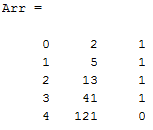
\includegraphics[scale=0.9]{H3-1}
\caption{Result of Matlab script}
\label{fig:prob1}
\end{figure}
This shows, that $f(4) \not=$ prime.


\section*{Problem 2}
\textbf{Let $a,b \in \mathbb{Z}$. Disprove the statement; if $a\cdot b$ then $(a+b)^2$ are of opposite parity, then $a^2b^2$ and $a+ab+b$ are of opposite parity.}
\\
\\
To disprove this we have to make a counterexample where you can start by saying $a=1, b=1$ and then $a=1, b=2$.
To minimize time spend doing this and making a general solution for this, we make the following Matlab script:

\begin{lstlisting}[caption=Problem 2, style=Code-Java, label=lst:prob2]
arrSize=5;
Arr = zeros(arrSize, 5);
a=1;
for i = 1:arrSize
    b=i;
   Arr(i,1)=a*b;
   Arr(i,2)=(a+b)^2;
   Arr(i,3)= a^2*b^2;
   Arr(i,4)=a+a*b+b;
   c = mod(Arr(i,1),2) ~= mod(Arr(i,2),2);
   d = mod(Arr(i,3),2) ~= mod(Arr(i,4),2);
   if c == d
       Arr(i,5)=0;
   else
       Arr(i,5)=1;
   end
end

Arr
\end{lstlisting}
Which gives us the result in Figure \ref{fig:prob2}, where column 1 is $a\cdot b$, column 2 is $(a+b)^2$, column 3 is $a^2b^2$, column 4 is $a+ab+b$ and column 5 is whether the first two columns are not same parity and the next two columns are not same parity (1 indeicate 'no').
\begin{figure}[hbtp]
\centering
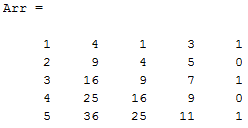
\includegraphics[scale=0.9]{H3-2}
\caption{Result of Matlab script}
\label{fig:prob2}
\end{figure}
This is only the first 5 combinations, where $a=1$ and \textit{b} runs from 1 to 5.
If $a=1, b=1$ the counterexample is shown.



\section*{Problem 3}
\textbf{Let $x, y \in \mathbb{R}^{+}$. Use a proof by contradiction to prove that if $x<y$ then $\sqrt{x} < \sqrt{y}$}
\\
\\
Lets rewrite the statement:
\begin{align}
\forall x, y \in \mathbb{R}^+, &P \Rightarrow Q & P = x < y \text{ and } Q = \sqrt{x}<\sqrt{y} \\
\exists x, y \in \mathbb{R}^+, &P \Rightarrow \neg Q \\
\neg Q &= \neg(\sqrt{x} < \sqrt{y})\\
\neg\sqrt{x} &< \neg \sqrt{y} \\
\sqrt{x} &\geq \sqrt{y} & \text{Remove negation}\\
x &\geq y & \text{Square both sides}
\end{align}

Since $x<y$ and $x\geq y$ is clearly not the same, the statement is proven.


\section*{Problem 4}
\textbf{Prove that there is no largest negative rational number. (Note: -1 is larger than -2.)}
\\
\\
A rational number is defined by $\mathbb{Q}: \{ \frac{a}{b}:a, b \in (\mathbb{Q} \cup \mathbb{Z})\}$.
By increasing \textit{b} and letting \textit{a} be a negativ number the number will be higher and higher but you can always find a higher number.
\[ \dfrac{-a}{b} < \dfrac{-a}{b+1}\]



\section*{Problem 5}
\textbf{Prove that there exits no positive integer \textit{x} such that $2x < x^2 < 3x$}
\\
\\
To prove there exist no positive integer, we can reduce the statement:
\begin{align}
2x < x^2 < 3x & \quad \text{Divide by } x\\
2 < x < 3 \label{equ:p5}
\end{align}
Since there exist no integer in Equation (\ref{equ:p5}) between 2 and 3, the statement is proven.



\section*{Problem 6}
\textbf{Prove that if \textit{n} is an odd integer, then $7n-5$ is even by}
\begin{enumerate}[a]
\item \textbf{direct proof}
\begin{itemize}
\item  Since an odd number, \textit{n}, times another odd numner, 7, is odd, substracting a thrid odd number, 5, will give an even number.
\item It can also be shown as follow:
\begin{align}
n&=odd\\
P(n)&=7(2x+1)-5\\
	&=14x+7-5\\
	&=2(x+2)\\
	&=2k
\end{align}
\end{itemize}
\item \textbf{proof by contrapositive}
\item[] What this means is, that if we can find an equation that states \textit{n} cannot be odd:
\item[]
\begin{align}
2x+1 &= 7 n-5 & \text{Try letting the equation be odd}\\
2x+6 &= 7n\\
2(x+3)&=7n & \text{Subtract }-6n \text{ on both sides}\\
2(x+3)-6n &= n &\text{Find the form } 2(a-n) = n\\
2(x+3-3n) &= n
\end{align}
\item[] If we tried to solve the left side and get an odd number, we will fail.
No \textit{x} will give us a left side which is odd.
Therefor \textit{n} is even.
\item \textbf{proof by contradiction}
\item[] This will give "\textit{n} is an odd integer, and $7n-5$ is odd"
\begin{align}
n&=even\\
P(n)&=7(2x)-5\\
	&=14x-5\\
	&=2(7x-2)-1\\
	&=2k-1 \label{equ:6}
\end{align}
\end{enumerate}
Equation(\ref{equ:6}) shows the contradiction is true and thereby the original statement is true.


\section*{Problem 7}
\textbf{Show that there exit two distinct irrational numbers \textit{a} and \textit{b} such that $a^b$ is rational.}
\\
\\
Example: 
\begin{align}
a &= \sqrt{2}^{\sqrt{2}}\\
b &= \sqrt{2}\\
a^b &= {\sqrt{2}^{\sqrt{2}}}^{\sqrt{2}}\\
a^b &= 2 \label{equ:7}
\end{align}
It has now been proven with Equation(\ref{equ:7}).



\section*{Problem 8}
\textbf{Disprove the statement: There is an integer \textit{n} such that $n^4+n^3+n^2+n$ is odd.}
\\
\\
To disprove this we look at the what $n^x$ is equal to:
\begin{align}
n^4+n^3+n^2+n &\Leftrightarrow n(n+1)\Big(n^2+1\Big) & \text{Factor via WolframAlpha}\\
\end{align}
Case 1: \textit{n} is even and has the form $2a$:
\begin{align}
n(n+1)\Big(n^2+1\Big) &= (2k)(2k+1)\Big((2k)^2+1\Big)\\
	&=\Big(4k^2+2k\Big)\Big(4k^2+1\Big)\\
	&=16k^4+4k^2+8k^3+2k\\
	&=2\Big(8k^4+4k^3+2k^2+k\Big)\\
	&=2a
\end{align}
The form is $2a$ which shows us, that if the input is even it will com out even.
\\
Case 2: \textit{n} is odd and has the form $2a+1$:
\begin{align}
n(n+1)\Big(n^2+1\Big) &= (2k+1)(2k+1+1)\Big((2k+1)^2+1\Big)\\
	&=\Big(4k^2+4k+1\Big)\Big(4k^2+1+4k+1\Big)\\
	&=16k^2+16k^3+8k^2+4k^3+16k^2+8k+4k^2+4k+2\\
	&=20k^3+44k^2+12k+2\\
	&=2\Big(10k^3+22k^2+6k+1\Big)\\
	&=2a
\end{align}
The form is again $2a$ which shows us, that if the input is odd it will come out even.
\\
It is now shown, that no matter the input parity, the output is even and thereby disproving the statement.

\end{document}